% !TEX root = ../my-thesis.tex
%
\chapter{The masses and dynamics of star clusters in the Milky Way}
\label{sec:dynamics}

\cleanchapterquote{Things are only impossible until they're not.}{Jean-Luc Picard}{(2364)}

\authorship{The results presented in this chapter will be published in Hunt and Reffert (\emph{in prep.}). All calculations, figures, and writing in this chapter were conducted by myself.}

% -------------------------------------
\section{Introduction}
\label{sec:dynamics:introduction}

Five years on since the release of \gaia\ DR2 \citep{brown_gaia_2018}, the census of open clusters (OCs) has been resoundingly overhauled \citep{cantat-gaudin_milky_2022}. Thousands of new objects have been discovered \citep[e.g.][]{liu_catalog_2019,castro-ginard_hunting_2020}, parameters have been determined to previously impossible levels of accuracy \citep[e.g.][]{bossini_age_2019,cantat-gaudin_painting_2020}, and many OCs reported before \gaia\ have been ruled out as asterisms \citep{cantat-gaudin_clusters_2020,piatti_assessing_2023,hunt_improving_2021,hunt_improving_open_2023}. However, the OC census in the age of \gaia\ remains far from perfect, and one resoundingly large issue stands out that I will attempt to address in this chapter: there is no robust observational criteria or definition for what an OC actually is \citep{hunt_improving_open_2023}.

Following up from the first major catalogue of OCs in the \gaia\ era \citep{cantat-gaudin_gaia_2018}, \cite{cantat-gaudin_clusters_2020} conducted a search for OCs that remained undetected in \gaia\ data, and created a set of empirical observational criteria intended to split dubious objects apart from OCs. This included recommendations that a candidate OC is a clear overdensity with at least $\sim10$ member stars, a colour-magnitude diagram (CMD) that follows a clear isochrone, a median radius $r_{50}$ smaller than 15~pc, and a proper motion dispersion corresponding to an upper limit no greater than 5~km\,s\textsuperscript{-1}. In their work, they used these criteria to show that a number of objects were highly likely to be asterisms.

In \cite{hunt_improving_open_2023} (hereafter Paper 2), we constructed the largest catalogue of OCs to date from a blind search of \gaia\ DR3 data \citep{gaia_collaboration_gaia_2022}. However, we found that the \cite{cantat-gaudin_clusters_2020} observational criteria were too permissive. Many of the objects we detected that passed these criteria were visually much more reminiscent of moving groups (MGs), with sparse, flat distributions that do not resemble the clustered nature of reliable, gravitationally bound OCs. In turn, this creates an awkward situation where our Paper 2 catalogue is challenging to use in many respects, with simple queries of the catalogue returning mostly MGs -- particularly within a few hundred pc of the Sun where MGs are most common. It is clear that a more precise method to distinguish between bound OCs and unbound MGs is required. 

It appears that the radius and proper motion constraints presented in \cite{cantat-gaudin_clusters_2020} are the primary area of the OC observational definition that requires improvement. Recalling Eqns.~\ref{eqn:intro:jacobi_radius}~and~\ref{eqn:intro:virial_ratio}, in addition to the theory around bound and unbound star clusters discussed in works such as \cite{portegies_zwart_young_2010} or \cite{krause_physics_2020}, one can note that a cluster's mass, radius, and velocity dispersion form a three-way link in defining the dynamical status of a star cluster. Simple individual cuts on radius, dispersion, or even cluster mass should be insufficient to accurately split OCs from MGs.

For example, consider a cluster at the upper end of allowed radii from the cuts of \cite{cantat-gaudin_clusters_2020}, with $r_{50}=15$~pc. Assuming $2 \, r_{50}\approx r_t$ for convenience (which is a fair approximation for most OCs), Eqn.~\ref{eqn:intro:jacobi_radius} predicts that in the solar neighbourhood, a cluster of this size would require a total mass of $\sim10^4$~\MSun\ in order to be a bound object with a Jacobi radius of this size -- a mass so high that it corresponds to some of the largest known young clusters in the Milky Way \citep{portegies_zwart_young_2010,cantat-gaudin_milky_2022}. Such a high mass appears unrealistic for the many small, sparse new clusters we detected in the solar neighbourhood in Paper 2. 

On the other hand, the proper motion dispersion upper limit from \cite{cantat-gaudin_clusters_2020} (corresponding to 5~\kms\ when converted to velocity dispersions) is also likely to be much too high for many clusters. Many of the moving groups we detected in Paper 2 have proper motion dispersions that, when converted to velocity dispersions, correspond to dispersions in the range of 1 to 4~\kms. Even with a relatively small $r_{50}$ of 1~pc, a cluster with a velocity dispersion of 2~\kms\ would need to have a mass of $\sim10^4$~\MSun\ to be in virial equilibrium, which once again would be a high mass for an OC in the Milky Way -- let alone within a few hundred pc of the Sun. 

These rough estimates suggest that analysis of OC masses and dynamics could be fruitful in attempting to discern between bound OCs and unbound MGs, as it is likely that the empirical cuts presented in \cite{cantat-gaudin_clusters_2020} are too high for most objects. In this chapter, I hence aim to refine the observational definition of OCs. By measuring the masses, Jacobi radii, and dynamics of star clusters in our catalogue from Paper 2, I aim to determine more accurately which objects are compatible with bound OCs. 

In Sect.~\ref{sec:dynamics:masses}, I outline a pipeline to calculate accurate cluster masses, including correcting for three different selection effects. Section~\ref{sec:dynamics:velocities} outlines my method to infer velocity dispersions from cluster proper motions. Section~\ref{sec:dynamics:results} outlines the mass, radius, and dispersion results of this work, including discussing the validity of velocity dispersions given potential binary star contamination. I discuss the results of this work further in Sect.~\ref{sec:dynamics:discussion}, including estimating the total number of OCs and MGs in the catalogue and estimating the mass-dependent completeness of the \gaia\ DR3 OC census. Finally, I briefly conclude this work in Sect.~\ref{sec:dynamics:conclusion}.

% PLAN
% - Masses are useful! Dynamics are useful! They're comparable to theory and represent measurements of fundamental (physical) parameters of OCs.
% - BUT: very limited measurements so far of these parameters.
% - Difficult to define OCs robustly without them (Hunt & Reffert 2023)
% - Empirical cuts on parameters insufficient to measure them.
% - MASSES: can be measured more or less two ways: counting stars or tidal parameters
% - discuss pros and cons of each way
% - DYNAMICS: some progress in studying for OCs in MW, but generally for small numbers of clusters only.
% - most clusters found to be supervirial. really?? what about as function of cluster mass, age, etc?
% - finally: masses useful for e.g. analysis of sample completeness. is a more fundamental physical parameter than the observed number of stars
% - give overview of what's in this chapter
% - emphasise that I'll be 


% -------------------------------------
\section{Mass and radius calculations}
\label{sec:dynamics:masses}

At the time of writing, there exists no large catalogue of OC masses derived using \gaia\ data, with the largest study to date including only 78 of the many thousands of OCs in the Milky Way \citep{cordoni_photometric_binaries_2023}. In this section, I outline a method to accurately derive photometric masses of a given cluster of stars detected in \gaia, including accounting for a range of selection effects. Then, this mass determination method is used to determine the most likely Jacobi radius of every cluster.

% PLAN
% - give a quick overview of what's in this methods section

\subsection{Inference of stellar primary masses}
\label{sec:dynamics:masses:isochrones}

\begin{figure}[t]
    \centering
    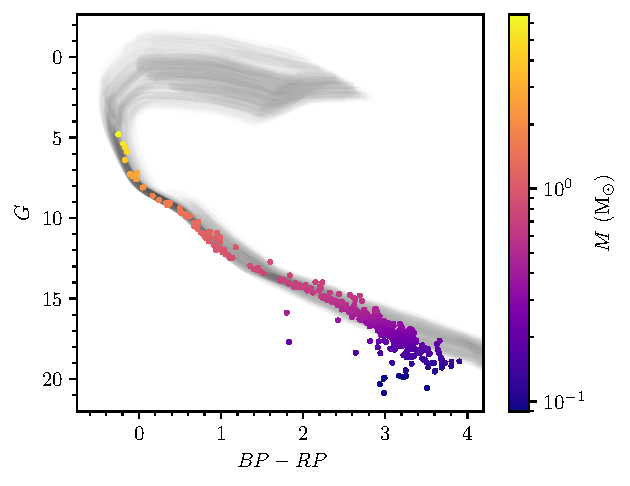
\includegraphics[width=0.8\textwidth]{fig/c4/masses_stellar.pdf}
    \caption[CMD of NGC~2451A with stars shaded by their median sampled stellar mass]{CMD of NGC~2451A with stars shaded by their median sampled stellar mass from interpolation against cluster isochrones. 100 isochrones sampled from the age-determination neural network in Paper 2 are plotted in black.}
    \label{fig:dynamics:masses:stellar_masses}
 \end{figure}

 The first step in deriving the photometric mass of a cluster requires calculating the masses of the cluster's member stars. To do so, I follow a similar method to those as used in numerous other works, such as \cite{meingast_extended_2021} and \cite{cordoni_photometric_binaries_2023}.

Using isochrone fits from Paper 2 and assuming solar metallicity for all clusters, PARSEC isochrones \citep{bressan_parsec_2012} were interpolated to predict mass as a function of G-band magnitude, $m(G)$. In general, this is sufficient for most member stars within clusters, and derives the most accurate stellar mass given \gaia\ G-band photometry and other calculated cluster parameters. 
 
However, particularly for older clusters, many clusters have giant stars beyond the turn-off point that dip below the tip of the main sequence (see Fig.~\ref{fig:intro:history:isochrones}), meaning that a single value of $G$ can correspond to multiple different stellar masses $m$. Hence, for isochrones where a direct conversion from magnitude to stellar mass is not possible for all stars, the interpolation region was split into a main sequence and turn-off point component. For stars near to and above the turn-off point, $BP-RP$ colours were also used to select the best fitting stellar mass. I do not use colours across the entire isochrone as \gaia\ DR3 colours can be under-estimated for stars fainter than $G\sim19$ \citep[especially in the BP band,][]{riello_gaia_2021}, and it is hence likely to be more accurate to limit the use of colour information in stellar mass interpolation as much as possible.

Since the age inference neural network from Paper 2 used variational inference to incorporate uncertainties, it can be sampled to produce multiple estimates on parameters for each cluster. Hence, for every cluster, the stellar mass interpolation process was repeated 100 times, allowing the uncertainty inherent from age and extinction determination to be incorporated into the stellar masses stochastically. Figure~\ref{fig:dynamics:masses:stellar_masses} shows the CMD of NGC~2451A, with its member stars shaded by their median sampled stellar mass and the 100 isochrone samples plotted in the background.

As this interpolation process does not account for binaries, these stellar masses can be considered as being roughly equal to the stellar mass of the primary stars of any binary system. A separate correction for binaries is discussed and added later in Sect.~\ref{sec:dynamics:masses:binaries}.


\subsection{Correction for selection effects}
\label{sec:dynamics:masses:selection}

Next, it is important to correct for selection effects. In Paper 2, we derived cluster membership lists down to magnitudes as faint as $G\sim20$. However, particularly at the faint end, clusters still become increasingly incomplete. This depends strongly on the position of the cluster in the disk: in the most extreme cases, for clusters in regions with high numbers of sources (such as towards the galactic centre), incompleteness is clear from magnitudes as bright as $G=17$. It is clear that accurate determination of cluster masses will require incorporation of these effects. The selection function of \gaia\ and subsamples of it have been relatively well studied in works such as \cite{boubert_completeness_2020-1}, \cite{boubert_completeness_2020}, \cite{rix_selection_functions_2021}, \cite{cantat-gaudin_empirical_model_2023}, and \cite{castro-ginard_estimating_selection_2023}, whose work I will adapt in this section to calculate star cluster selection functions.

The incompleteness of a cluster's membership list in Paper 2 is governed by three primary effects. Firstly, there is the simple probability that a source with attributes $\vec{q}=\left\{ l,b,G,... \right\}$ appears in the \gaia\ catalogue at all, $S_C^\text{parent}(\vec{q})$. To compute this, I use the selection function presented in \cite{cantat-gaudin_empirical_model_2023}, who compared the \gaia\ catalogue with deep photometric surveys of the galactic disk and globular clusters, deriving $S_C^\text{parent}(\vec{q})$ empirically as a function of the position and magnitude of a source for the entire \gaia\ DR3 catalogue. This builds on the purely theoretical \gaia\ selection function derived in \cite{boubert_completeness_2020-1} and \cite{boubert_completeness_2020}. 

However, many of the sources in \gaia\ do not include proper motions and parallaxes, do not include full photometry, or do not have reliable astrometry. Our Paper 2 membership lists were computed for a subsample of \gaia\ sources: namely, those with five or six parameter astrometric solutions, $G$, $BP$, and $RP$ photometry, and a \cite{rybizki_classifier_2022} v1 quality flag greater than 0.5, indicating that the source is likely to have reliable astrometry. This constitutes a subsample of 729~million stars from the overall \gaia\ DR3 catalogue.

To compute the probability that a source appears in this subsample given that it is also in the parent \gaia\ catalogue, i.e. $S_C^\text{subsample}(\vec{q} \mid \vec{q}\text{ in parent})$, I use the method outlined in \cite{castro-ginard_estimating_selection_2023} and based on \cite{rix_selection_functions_2021}. Firstly, sources are binned based on their attributes $\vec{q}$. Then, within bins, the chance that a source with attributes $\vec{q}$ appears in the subsample is modelled as a binomial distribution $\mathcal{B}(n,\,p)$, where $n$ is the number of sources in the \gaia\ catalogue in this bin with attributes $\vec{q}$ and $p$ is the probability that a source with these attributes makes it into the subsample of valid stars. In practice, $p$ is unknown; hence, an uninformative uniform Beta distribution prior on $p$ given the number of observed sources in the bin is used \citep[for full methodology, see][]{castro-ginard_estimating_selection_2023}.

In practice, one must choose the attributes $\vec{q'}$ on which the selection function is assumed to depend. The subsample of stars we use is almost entirely dependent on astrometric quality. The astrometric quality of \gaia\ is strongly correlated with sky position and G-band magnitude, corresponding to background star density, the number of scans of a given position by the \gaia\ telescope, and the brightness (signal-to-noise ratio) of a source \citep{lindegren_gaia_2021}. Hence, I compute $S_C^\text{subsample}(\vec{q} \mid \vec{q}\text{ in parent})$ as a function of position and magnitude, selecting a region corresponding roughly to the on-sky extent of a cluster for consideration and binning sources in bins of size $0.2$~mag. Bins were expanded until every bin contained at least ten sources, ensuring that no range of the selection function was under-sampled, but while preserving high resolution between $11 < G < 20$ where most sources in \gaia\ are.

Finally, I also found that the selection function of star cluster membership lists could depend on effects due to our adopted clustering algorithm and methodology in Paper~2, which is the probability that a given source is assigned as a member of a cluster by our clustering algorithm given that it appears in the subsample of valid sources considered for clustering analysis, $S_C^\text{algorithm}(\vec{q} \mid \vec{q}\text{ in subsample})$. Especially at high distances or within crowded fields, cluster proper motions and parallaxes become relatively uninformative, with many cluster members becoming relatively indistinguishable from field stars in these axes of \gaia\ astrometry. For distant clusters such as King~9, which is at a distance of $\sim6$~kpc, this can have a strong effect on our membership lists. Our adopted clustering algorithm from Paper 2, HDBSCAN, is density-based -- meaning that members are only assigned to a given cluster if they increase the contrast of a given cluster against unclustered stars. In practice, this means that stars away from the mean cluster proper motion or parallax are less likely to be assigned as cluster members, with many being missed in the worst cases. This is particularly dominant for faint sources at which \gaia\ astrometric errors can be on the order of (or even larger than) our measured cluster proper motion and parallax dispersions, meaning that many member stars are likely missed for the most distant objects. Errors on positions are correspondingly negligible compared to the generally no smaller than $0.1^\circ$ size of clusters, and so this effect is only of concern for cluster proper motions and parallaxes.

\begin{figure}[p]
    \centering
    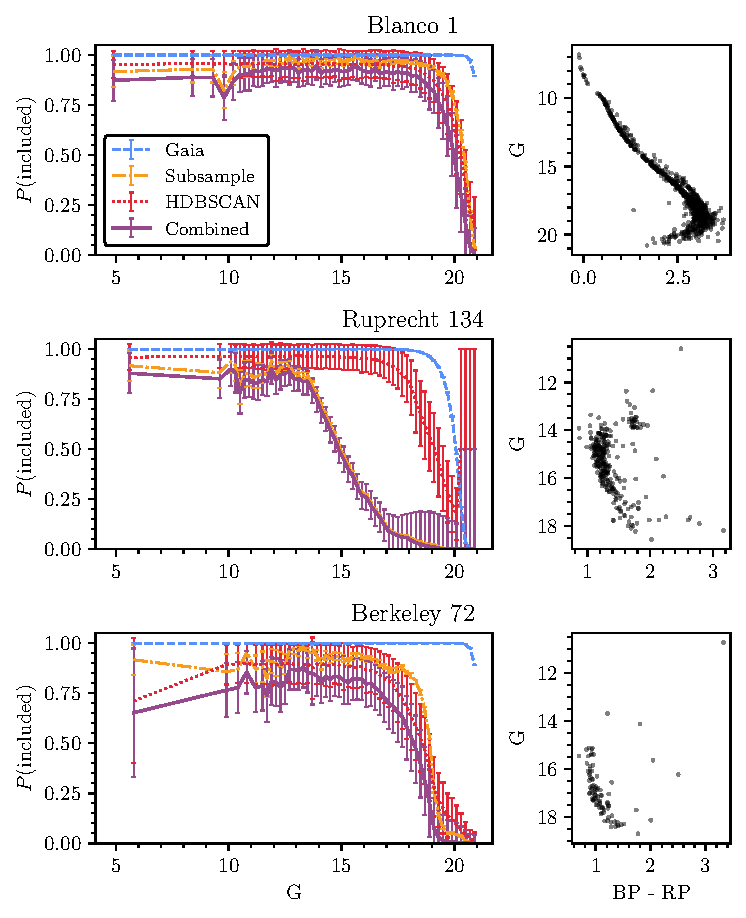
\includegraphics[width=\textwidth]{fig/c4/mass_selection_functions.pdf}
    \caption[Estimated cluster selection functions for three OCs from Paper~2: Blanco~1, Ruprecht~134, and Berkeley~72]{Estimated cluster selection functions for three OCs from Paper~2: Blanco~1, Ruprecht~134, and Berkeley~72. The left column shows computed cluster selection functions and a combined cluster selection function after accounting for all three dominant selection effects. The right column shows the CMD of each considered cluster for comparison.}
    \label{fig:dynamics:masses:selection_effects}
\end{figure}

To model this effect, I developed a novel stochastic technique to simulate the probability that a source would have mean \gaia\ astrometry within the detected HDBSCAN cluster. Firstly, the cluster detected by HDBSCAN is modelled as a three-dimensional ellipsoid in proper motion and parallax space. Then, 100\,000 stars with magnitudes uniformly distributed in the range $2 < G < 21$ were simulated, with astrometric errors assigned to each star depending on the error distribution of sources in the on-sky vicinity of a cluster. For each star, ten mean astrometric positions were simulated, given its simulated \gaia\ astrometric errors which form a multivariate normal distribution in proper motion and parallax space. For each simulation, a mean astrometric position within the cluster ellipsoid is assumed to be assigned as a cluster member, and a star whose mean astrometric position is outside the cluster ellipsoid is assumed to be assigned as a non-member. The results of these simulations for each cluster are binned using the same bins as the subsample selection function, and are then combined into an estimated per-cluster clustering algorithm selection function as a function of G-band magnitude. Poisson uncertainties are computed as the uncertainties on these bins.

Finally, all three independent selection effects are multiplied together, giving the total cluster selection function $S_C^\text{cluster}$:

\begin{equation}
    S_C^\text{cluster} = 
    S_C^\text{parent}(\vec{q})
    \cdot
    S_C^\text{subsample}(\vec{q} \mid \vec{q}\text{ in parent})
    \cdot
    S_C^\text{algorithm}(\vec{q} \mid \vec{q}\text{ in subsample}).
    \label{eqn:dynamics:masses:selection_function}
\end{equation}

Figure~\ref{fig:dynamics:masses:selection_effects} shows the computed cluster selection functions for three OCs: Blanco~1, Ruprecht~134, and Berkeley~72. Blanco~1 is a nearby ($d\approx240$~pc), high galactic latitude OC that suffers minimally from background crowding and is easy to separate from field stars. Its selection function is mostly complete down to $G\sim19$. On the other hand, Ruprecht~134 is an older, more distant cluster ($d\approx2.3$~kpc) that is in one of the densest regions of the galactic disk, with $l=0.3^\circ$ and $b=-1.6^\circ$. It is probably one of the most incomplete clusters in our entire catalogue. Its incompleteness is mostly due to the subsample selection function, as many sources do not have high enough quality \gaia\ astrometry to be included in our subsample of considered sources. Finally, Berkeley~72 is a distant, smaller cluster ($d\approx5.1$~kpc) whose members are more difficult to separate from field stars. Like many distant objects, the selection function of Berkeley~72 appears mostly dominated by the selection function of our clustering algorithm from Paper~2 when applied with our methodology. 

It is also worth noting that in general, no clusters appear to have a range in $G$ in which their CMD is 100\% complete. Many of these missing stars across all magnitudes are likely to be binaries. Other than for a small subsample of around 1~million sources, \gaia\ DR3 astrometric fits assume that each source is a single star. Hence, binaries with deviations large enough to be detectable by \gaia\ can have poor-quality astrometric fits, resulting in high reduced $\chi^2$ values and high error astrometry that is rejected by quality cuts such as the one used for our subsample of stars \citep[][; see also Sect.~\ref{sec:intro:history:gaia:background}]{lindegren_gaia_2021}.



\subsection{Correction for unresolved binaries}
\label{sec:dynamics:masses:binaries}

Given that the stellar mass inference in Sect.~\ref{sec:dynamics:masses:selection} only calculated the masses of stellar primaries, assuming in the process that every star is single, it is important to also correct for an additional increase to cluster mass functions due to unresolved binaries.

Recently, measurements of the binary star fraction in a number of clusters have been made using \gaia\ DR3 photometry, with \cite{cordoni_photometric_binaries_2023} measuring this for 78 reliable OCs and \cite{donada_multiplicity_fraction_2023} measuring this for 202 OCs within 1.5~kpc. Both works are only able to measure the binary star fraction down to mass ratios of $q\approx0.6$, noting that it becomes difficult to disentangle lower mass ratio binaries from the main sequence of single stars, particularly for clusters with differential extinction. Given that the mass ratio distribution of binaries in the field has been shown to peak around $q\sim0.3$ \citep{moe_mind_2017}, it is hence unlikely to be possible using \gaia\ DR3 photometry alone to accurately measure the full mass ratio distribution of unresolved and resolved binary stars within a cluster, let alone across a large sample of clusters such as the 7167 in our catalogue from Paper 2.

For now, I use the selection effect corrected relations for multiplicity fraction, companion star frequency, and mass ratio of field stars from \cite{moe_mind_2017} to apply binary star corrections to each cluster mass bin. In addition, to calculate the fraction of unresolved to resolved binary stars, simulations of clusters and the astrometry of binary stars assuming the period and eccentricity distributions from \cite{moe_mind_2017} were conducted using \texttt{SPISEA} \citep{hosek_jr_pypopstar_2020} and \texttt{astromet} \citep{penoyre_astrometric_2022,penoyre_astrometric_2022-1}, with a binary correction being applied proportional to however many resolved or unresolved binaries were expected for each cluster.

Incorporation of these binary star corrections results in cluster mass bins that are inflated by around 10\% to 30\%, depending on the distance of the cluster and how many of its stars are likely to be in unresolved or resolved binaries. Uncertainties around binary star fraction likely add an up to 30\% additional uncertainty on my derived cluster masses, since a single relation is applied to all clusters. 

Before the final publication of this chapter in a paper, it may be possible to improve this binary star correction further. However, this simple correction may already be sufficient, since determination of the binary star fraction across all mass ratios for all (or even $\sim5$\%) of the 7167 clusters is not feasible with current available data.


\subsection{Mass function fits}
\label{sec:dynamics:masses:imf_fits}

\begin{figure}[p]
    \centering
    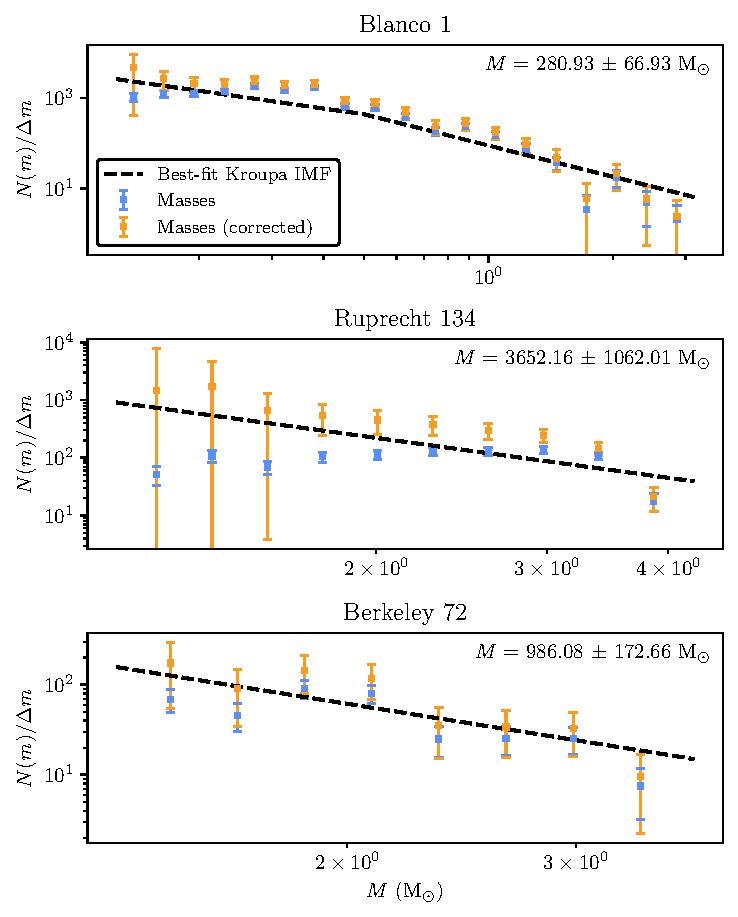
\includegraphics[width=\textwidth]{fig/c4/mass_functions.pdf}
    \caption[Mass function fits to the three OCs from Fig.~\ref{fig:dynamics:masses:selection_effects}]{Mass function fits to the three OCs from Fig.~\ref{fig:dynamics:masses:selection_effects}. The blue points show measured binned stellar masses, the orange points show these masses after correcting for selection effects and modest assumptions about binary stars, and the black dashed line shows the best-fitting Kroupa IMF. The integral of the cluster mass function is written in the top right of each plot.}
    \label{fig:dynamics:masses:mass_functions}
\end{figure}

Having calculated accurate completeness and binary-corrected mass bins for every cluster, I next used these mass measurements to calculate the total mass of every cluster. To do so, I fit a \cite{kroupa_variation_2001} initial mass function (hereafter Kroupa IMF) to the mass function of each cluster using least squares fitting. The integral of the Kroupa IMF from 0.03~\MSun to the highest observed stellar mass in the cluster is then taken as the mass value for the cluster.

One could also fit bespoke mass functions to each cluster \citep[e.g. as in][]{cordoni_photometric_binaries_2023}. The IMF is known to be well approximated by a broken power law for most populations, with a break point around 0.5~\MSun \citep{kroupa_variation_2001}. However, low masses are poorly resolved for many of the clusters in our sample, with clusters more distant than $\sim1$~kpc or clusters with reddening values $A_V \gtrsim 2$ having few or no stars at masses lower than 0.5~\MSun. Hence, it would not be possible to fit a two-part mass function to these clusters, preventing an accurate estimate of their true total mass. The `safer' option in this case is to fit Kroupa IMFs to all clusters, deriving masses on the same scale with the same assumed mass function.

Some N-body simulations have suggested that cluster mass functions become depleted of low mass stars over time, due to lower mass stars being preferentially ejected from clusters \citep{krause_physics_2020}. Before publishing this work, it may also be insightful to fit bespoke mass functions to nearby clusters to investigate this effect. However, this would likely also require a better determination of a binary star mass function correction for each cluster, which may be beyond the scope of this work.

Figure~\ref{fig:dynamics:masses:mass_functions} shows mass function fits to the three clusters from Fig.~\ref{fig:dynamics:masses:selection_effects}. Generally, Kroupa IMFs are a reasonable approximation for most clusters, and the integral of these mass functions produces reasonable values of the total mass for each cluster. 

More work should be done to improve the fitting process of cluster mass functions before publication. One can see in Fig.~\ref{fig:dynamics:masses:mass_functions} that outlier points can over-constrain fits and result in erroneously higher or lower masses (such as the highest mass bin for Ruprecht~134, or some of the higher mass bins for Blanco~1 -- in both cases, these reduce the final total cluster mass by a large amount). I intend to upgrade the least squared fitting of cluster mass functions to use a more statistical approach that includes rejection of outlier points, which should improve the overall accuracy of derived cluster masses.


\subsection{Jacobi radius inference}
\label{sec:dynamics:masses:jacobi}

\begin{figure}[t]
    \centering
    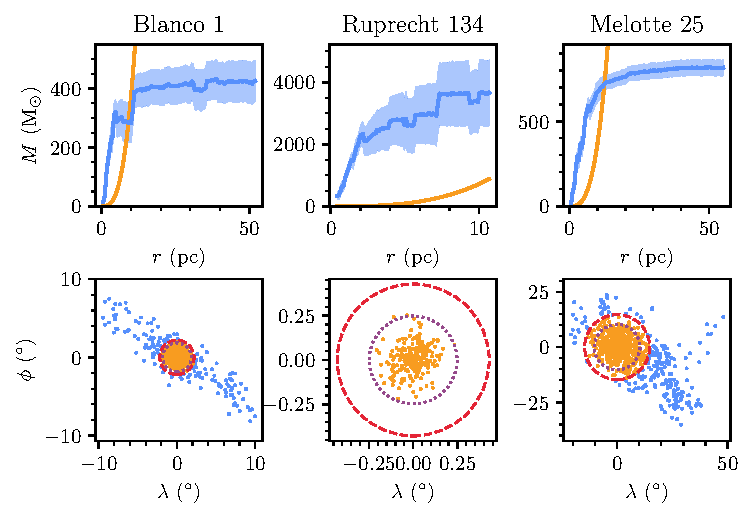
\includegraphics[width=\textwidth]{fig/c4/masses_jacobi_radii.pdf}
    \caption[Jacobi radius determination for three OCs: Blanco~1, Ruprecht~134, and Melotte~25]{Jacobi radius determination for three OCs: Blanco~1, Ruprecht~134, and Melotte~25 (the Hyades). Each of the three columns corresponds to each cluster. \emph{Top row:} the estimated total mass contained within a radius $r$ is shown in blue ($M_\text{obs}(r)$), with the $1\sigma$ error region shaded on the plot. The orange line shows the theoretical amount of mass contained within a radius $r$ according to the Jacobi radius equation ($M_J(r)$, Eqn.~\ref{eqn:intro:jacobi_radius}). The intersection of these two lines corresponds to the cluster's $r_J$. \emph{Bottom row:} the distribution of cluster member stars. To remove spherical distortions, positions are rotated to an arbitrary coordinate frame with longitude $\lambda$ and latitude $\phi$ centred on the cluster centre. Stars within $r_J$ are shown in orange while stars outside $r_J$ are shown in blue. The dashed red line shows $r_J$, while the dashed purple line corresponds to the approximate value of $r_t$ determined in Paper 2.}
    \label{fig:dynamics:masses:radii_examples}
\end{figure}

\begin{figure}[t]
    \centering
    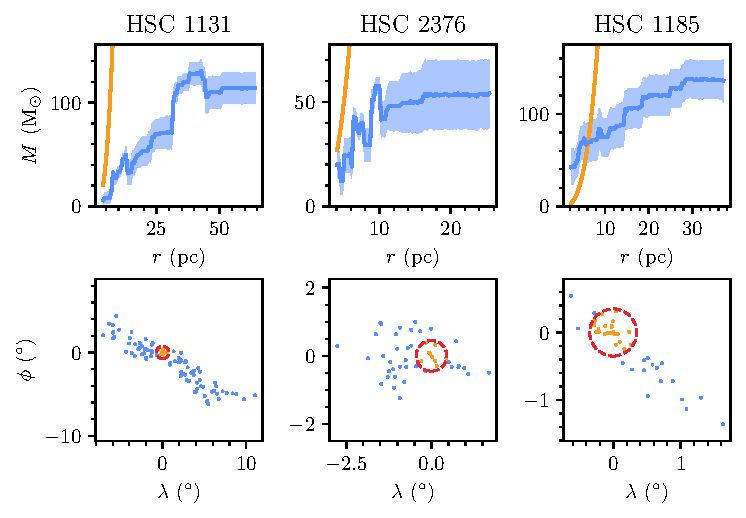
\includegraphics[width=\textwidth]{fig/c4/masses_jacobi_determination.pdf}
    \caption[Jacobi radius determination for three candidate new OCs from Paper 2 that were highlighted as example new objects]{Jacobi radius determination for three candidate new OCs from Paper 2 that were highlighted as example new objects (see Sect.~\ref{c3:sec:discussion-moving_groups} and Fig.~\ref{c3:fig:sus_clusters}). The plot is formatted the same as Fig.~\ref{fig:dynamics:masses:radii_examples}. The most likely Jacobi radius for HSC~1131 and HSC~2376 is shown, although $M_\text{obs}(r)<M_J(r)$ for all radii for both clusters, and they are hence more likely to be MGs (see text).}
    \label{fig:dynamics:masses:radii_examples_sus}
\end{figure}

Finally, having constructed a pipeline to calculate cluster masses, I used these methods to infer the Jacobi radius $r_J$ of the clusters in our sample. Recalling Sect.~\ref{sec:intro:theory:profile}, the Jacobi radius defines the radius within which a star cluster's gravitational potential is greater than the potential of its host galaxy. Within this radius, all stars have the potential to be bound together. I define the amount of mass within this radius as the Jacobi (or bound) mass $M_J$ of each cluster, and the total mass of all observed member stars (including tidal tails) as $M_A$.

The Jacobi radius of each cluster was calculated using the method of \cite{meingast_extended_2021}. Firstly, I calculated the circular and epicyclic frequencies at the cluster's distance from the galactic centre using \texttt{galpy} \citep{bovy_galpy_python_2015} and the \texttt{MWPotential2014} potential model defined in \cite{bovy_galpy_python_2015}. Next, for each cluster, the theoretical value of the Jacobi mass as a function of radius $M_J(r)$ was calculated at all radii outwards from the centre of the cluster. Finally, the observed cluster mass as a function of radius $M_\text{obs}(r)$ was calculated by repeating the process of binning stars by mass, applying a correction for unresolved binaries, and fitting Kroupa IMFs to the resulting cluster mass functions. The radius at which $M_\text{obs}(r) = M_J(r)$ is then hence the Jacobi radius of the cluster. Only radii at which the cluster would have at least ten observed bound members were considered, differentiating any potential bound cluster from multiple star systems and in accordance with common minimum limits on the size of an OC \citep{cantat-gaudin_clusters_2020,portegies_zwart_young_2010}.

There are two special cases of this method worth discussing. Firstly, for clusters without a valid Jacobi radius, $M_\text{obs}(r)<M_J(r)$ at all radii. These clusters can be considered to have no radius at which their potential is stronger than that of the Milky Way, and would be better classified as MGs instead of OCs. For these clusters, I take the radius at which they are closest to having a valid Jacobi radius and compute the probability of a cluster nevertheless having a valid Jacobi radius, given the uncertainties on their computed observed mass. For most clusters with $M_\text{obs}(r)<M_J(r)$ for all $r$, this probability is near zero; although some edge-case objects may still have a small chance of having a valid Jacobi radius. Secondly, some clusters have an observed mass greater than their Jacobi mass even at the highest angular distance of any member star from the cluster core. This is particularly common for more distant or difficult to detect clusters, and is likely because they do not have detected member stars out to their true $r_J$. For these clusters, I compute $r_J$ for the mass of the entire detected cluster, giving a Jacobi radius larger than the total extent of the cluster on the sky. This value is likely to be an under-estimate of the true cluster $r_J$ as the undetected outskirts of the cluster would increase $r_J$ further.

Figure~\ref{fig:dynamics:masses:radii_examples} shows $M_\text{obs}(r)$ and $M_J(r)$ for three clusters: Blanco~1, Ruprecht~134, and Melotte~25 (the Hyades), in addition to the member stars within these radii. Firstly, it can be noted that at $r<r_J$, $M_\text{obs}(r)$ is greater than $M_J(r)$ for Blanco~1 and Melotte~25, showing that these are reliable clusters with a range of radii where enough mass is present that the cluster's gravitational potential is stronger than that of the Milky Way. Ruprecht~134 is a more distant and difficult to detect cluster for which $M_\text{obs}(r)$ is always greater than $M_J(r)$. The Jacobi radius of its total population is larger than the observed maximum radius of the cluster.

This method also appears to be a good test of whether an object is an OC or an MG. Figure~\ref{fig:dynamics:masses:radii_examples_sus} shows the Jacobi radius determination for three candidate OCs from Paper~2 that were highlighted as example new objects. In Sect.~\ref{c3:sec:discussion-moving_groups}, we suggested that HSC~1131 and HSC~2376 were sparse objects that appear more compatible with moving groups, and HSC~1185 is an object with a denser core that could be compatible with a small OC. Figure~\ref{fig:dynamics:masses:radii_examples_sus} suggests that this is the case: HSC~1131 and HSC~2376 both do not have a valid Jacobi radius, while HSC~1185 is compatible with a small cluster with around 65~\MSun\ of bound stellar content.

Finally, it is worth commenting on a remaining issue with this calculation that I hope to fix before publication. $M_\text{obs}(r)$ values in Figs.~\ref{fig:dynamics:masses:radii_examples}~and~\ref{fig:dynamics:masses:radii_examples_sus} often jump up and down. In addition, the fitted mass within a radius $r$ can even decrease as $r$ increases, as appears to be the case for Blanco~1. This is due to issues with mass function fitting identified in Sect.~\ref{sec:dynamics:masses:imf_fits}, which causes mass function fits to be unstable and biased by outlier mass bins. Improvements to mass function fitting should make this process more stable and should improve the accuracy of $r_J$ determination for all clusters.



% -------------------------------------
\section{Velocity dispersion inference}
\label{sec:dynamics:velocities}

While the derived cluster masses and Jacobi radii from the previous section are effective to determine which clusters have the possibility of being bound, the dynamical state of a cluster depends not only on its mass and radius, but also its velocity dispersion (Eqn.~\ref{eqn:intro:virial_ratio}). Velocity dispersions from \gaia\ data have been used in a number of works such as \cite{bravi_gaia-eso_2018}, \cite{kuhn_kinematics_2019}, and \cite{pang_3d_2021} to probe the current dynamical status of star clusters. % Even for clusters with a valid Jacobi radius, it may be that their velocity dispersion is so high that it is clear the cluster is a dense (but unbound) object. 

While some dynamical studies have used radial velocities to study the dynamics of OCs \citep[e.g.][]{bravi_gaia-eso_2018} or proper motions in combination with radial velocities \citep[e.g.][]{evans_mass_2022-1}, I aim to use exclusively proper motions \citep[e.g. as in][]{kuhn_kinematics_2019}, as they are the only measurement available reliably across the entire sample of clusters. Hence, in this section, I outline a method to derive approximate cluster velocity dispersions from cluster proper motions based on a simple Gaussian model.


\subsection{Gaussian velocity dispersion model}
\label{sec:dynamics:velocities:model}

\begin{figure}[t]
    \centering
    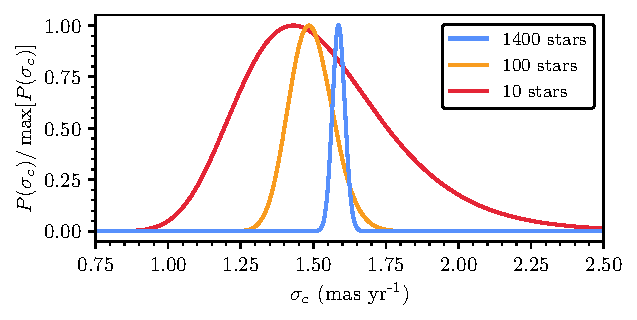
\includegraphics[width=\textwidth]{fig/c4/dispersion_pdf.pdf}
    \caption[Proper motion dispersion likelihood in Eqn.~\ref{eqn:dynamics:velocities:likelihood} evaluated for different subsets of stars in Melotte~22]{Proper motion dispersion likelihood in Eqn.~\ref{eqn:dynamics:velocities:likelihood} evaluated for different subsets of stars in Melotte~22 (the Pleiades). The blue curve shows all 1400 stars within my calculated value of $r_J$. The orange and red curves are for sets of 100 and 10 stars respectively that were randomly sampled from the overall cluster, showing how the likelihood becomes broader and asymmetric as uncertainty on the true value increases.}
    \label{fig:dynamics:velocities:pdfs}
\end{figure}

By definition, dynamically relaxed virialised clusters are expected to have an isothermal (Maxwellian) velocity dispersion that will be well described by a Gaussian \citep{king_structure_1966,portegies_zwart_young_2010}, assuming that stars within a cluster of $n$ stars have independent, uncorrelated velocities -- namely, that there is no overall axis of rotation within the cluster, and the cluster is well described by a \cite{king_structure_1966} profile. Hence, the assumption of a Gaussian model for the distribution of cluster proper motions is likely to be a good approximation for most OCs, and I approximate cluster velocity dispersions as a symmetrical multivariate Gaussian distribution with a single dispersion in all axes, $\sigma_c$.

Given the set of all proper motion measurements for stars within a cluster $\{\vec{\mu}\}$, which each have corresponding covariances from the set of all covariance matrices  $\{\Sigma\}$, and a mean cluster proper motion $\vec{\mu}_c = (\mu_{\alpha, c}, \mu_{\delta, c})$, the likelihood of the observed data given these cluster parameters is hence given by

\begin{equation}\label{eqn:dynamics:velocities:likelihood}
    \mathcal{L} 
    = P(\{\vec{\mu}\}\mid\vec{\mu}_c,\sigma_c,\{\Sigma\}).
\end{equation}

Every $i^{th}$ star in the cluster has a true proper motion $\vec{\bar{\mu}}_i~=~(\bar{\mu}_{\alpha,~i},\bar{\mu}_{\delta,~i})$, which is drawn from the two-dimensional Gaussian

\begin{equation}\label{eqn:dynamics:velocities:generative_model}
    P(\vec{\bar{\mu}}_i \mid
    \vec{\mu}_c, \sigma_c)_i \sim \mathcal{N}(\vec{\mu}_c \mid \sigma_c),
\end{equation}

\noindent
where $\mathcal{N}$ denotes a bivariate normal distribution.

However, \emph{Gaia} proper motion measurements have uncertainties, and the measured proper motion of every source $\vec{\mu}_i~=~(\mu_{\alpha,~i},~\mu_{\delta,~i})$ is the true proper motion $\vec{\bar{\mu}}_i$ convolved with Gaussian measurement uncertainties. $\vec{\mu}_i$ has a covariance matrix $\Sigma_i$ defined as:

\begin{equation}
    \Sigma_i = 
        \begin{bmatrix}
        \sigma_{\mu_\alpha, i}^2 
        & \rho_i \sigma_{\mu_\alpha, i} \sigma_{\mu_\delta, i}\\
        \rho_i \sigma_{\mu_\alpha, i} \sigma_{\mu_\delta, i}
        & \sigma_{\mu_\delta, i}^2
        \end{bmatrix}
\end{equation}

\noindent
where $\sigma_{\mu_\alpha, i}$ and $\sigma_{\mu_\delta, i}$ are the uncertainties on proper motions in right ascension and declination respectively, and $\rho_i$ is the covariance coefficient between them. Every measured proper motion $\vec{\mu}_i$ is therefore drawn from a bivariate normal distribution centred on the true proper motion of star $i$ $\vec{\bar{\mu}}_i$ as:

\begin{equation}\label{eqn:dynamics:velocities:measurement_model}
    P(\vec{\mu}_i \mid
    \vec{\bar{\mu}}_i, \Sigma_i)_i \sim \mathcal{N}(\vec{\bar{\mu}}_i \mid \Sigma_i),
\end{equation}

\noindent
which is the measurement model for each star which accounts for \emph{Gaia} astrometric uncertainties.

Since the true proper motion $\vec{\bar{\mu}}_i$ is unknown, all possible values of this parameter must be marginalised over to remove it from the likelihood and arrive at a final (solvable) equation. The final likelihood for each star is hence given by

\begin{equation}
    \mathcal{L}_i = P(\vec{\mu}_i \mid \vec{\mu}_c, \sigma_c, \Sigma)_i = 
    \int P(\vec{\mu}_i, \vec{\bar{\mu}}_i \mid \vec{\mu}_c, \sigma_c, \Sigma)_i \; d \vec{\bar{\mu}}_i.
\end{equation}

\noindent
Using the product rule and conditional independence between parameters, this can be expressed in terms of Eqns.~\ref{eqn:dynamics:velocities:generative_model}~and~\ref{eqn:dynamics:velocities:measurement_model} as:

\begin{equation}
    \mathcal{L}_i% = P(\vec{\mu}_i \mid \vec{\mu}_c, \sigma_c, \Sigma)_i
    = \int P(\vec{\mu}_i \mid \vec{\bar{\mu}}_i, \Sigma_i)_i \;
    P(\vec{\bar{\mu}}_i \mid \vec{\mu}_c, \sigma_c)_i \;
    d \vec{\bar{\mu}}_i.
\end{equation}

Finally, for all $n$ stars in the cluster, assuming that the set of all proper motion measurements $\{\vec{\mu}\}$ with corresponding covariances $\{\Sigma\}$ is independent, the final likelihood is given by:

\begin{equation}\label{eqn:dynamics:velocities:final_likelihood}
    \mathcal{L} 
    = P(\{\vec{\mu}\}\mid\vec{\mu}_c,\sigma_c,\{\Sigma\}) 
    = \prod_{i=1}^{n} \mathcal{L}_i.
\end{equation}

Evaluations of this likelihood for the Pleiades are shown in Fig.~\ref{fig:dynamics:velocities:binary_contamination}, as well as for smaller subsets of stars randomly sampled from the Pleiades. When the cluster dispersion is possible to measure precisely, the Eqn.~\ref{eqn:dynamics:velocities:likelihood} likelihood is symmetric; in less certain cases, the likelihood becomes asymmetric, with a long tail towards high $\sigma_c$ values.

In practice, \emph{Gaia} measurements are not strictly independent, and coordinate frame distortions due to effects such as the radial motion of the cluster will cause clusters to have distorted, non-Gaussian proper motion distributions. In the next section, I discuss how cluster proper motions are corrected for various distortions arising from spherical geometry and cluster radial velocity projected into the tangential proper motion plane.


\subsection{Coordinate frame and radial velocity corrections}
\label{sec:dynamics:velocities:correction}

Cluster proper motions are corrected in two ways. Firstly, I remove the impact of an effect known as `perspective expansion' due to the relative motion of a cluster to the Sun. Particularly for clusters with high radial velocities such as the Hyades, this effect can cause stars to appear to expand or contract away from the centre of the cluster \citep{kuhn_kinematics_2019}. To first order, this contributes an excess proper motion $\Delta \mu_{\alpha^*,i}$ and $\Delta \mu_{\delta,i}$ to star $i$ given by \citep{vanleeuwen_parallaxes_proper_2009}:

\begin{equation}
    \Delta \mu_{\alpha^*,i} \approx \Delta\alpha_i \left( 
        \mu_{\delta,c} \sin\delta_c - \frac{v_{r,c} \varpi_c}{k}\cos\delta_c
    \right)
\end{equation}

\begin{equation}
    \Delta \mu_{\delta} \approx -\Delta\alpha_i \mu_{\alpha^*,c} \sin\delta_c - \Delta\delta_i \frac{v_{r,c}\varpi_c}{k},
\end{equation}

\noindent
where $\alpha_c$, $\delta_c$, $\mu_{\alpha^*,c}$, $\mu_{\delta,c}$, and $\varpi_c$ are the astrometric parameters for the cluster derived in Paper~2, $\Delta\alpha_i$ and $\Delta\delta_i$ are the distance in right ascension and declination of the star from the cluster centre, $v_{r,c}$ is the cluster radial velocity determined in Paper~2, and $k$ is a constant equal to 4.74. For 1418 clusters with no determined radial velocity (which are generally distant and would be minimally affected by perspective expansion), this correction was not applied.

In addition, to remove any possible spherical distortions on cluster proper motions, I rotate the coordinate frame of astrometric measurements and associated proper motions into a frame centred on the cluster centre determined in Paper~2. Errors on proper motions are transformed to the new frame. For most clusters, the effect of this correction is negligible; however, for clusters near to the poles of the adopted coordinate frame, this correction prevents cluster proper motions from having a ring-like distribution.

\subsection{Inference procedure}
\label{sec:dynamics:velocities:inference}

Finally, cluster velocity dispersions were inferred for all clusters with a maximum likelihood method. Only stars within the identified Jacobi radius of each cluster were considered when inferring $\sigma_c$, which mostly removes the signature of cluster tidal tails from clusters. In addition, only stars with a renormalised unit weight error (RUWE) value of less than 1.4 were considered, which should help to restrict inference to only stars with reliable astrometry and should remove some obvious astrometric binaries \citep{lindegren_gaia_2021,penoyre_astrometric_2022,penoyre_astrometric_2022-1}.

The full PDF and associated confidence intervals around the most likely $\sigma_c$ value were determined. To marginalise over and integrate the likelihood in Eqn.~\ref{eqn:dynamics:velocities:likelihood} quickly for all sources, a \texttt{C++} program was written using the integration package in the GNU Scientific Library\footnote{\url{https://www.gnu.org/software/gsl/}}.


% -------------------------------------
\section{Masses, radii, and virial ratios for the entire sample of clusters}
\label{sec:dynamics:results}

In this section, I present an overview of the current results from my work into OC masses and dynamics. I begin with an overview of the cluster mass and Jacobi radius results.


\subsection{Masses and radii}
\label{sec:dynamics:results:masses}

\begin{figure}[p]
    \centering
    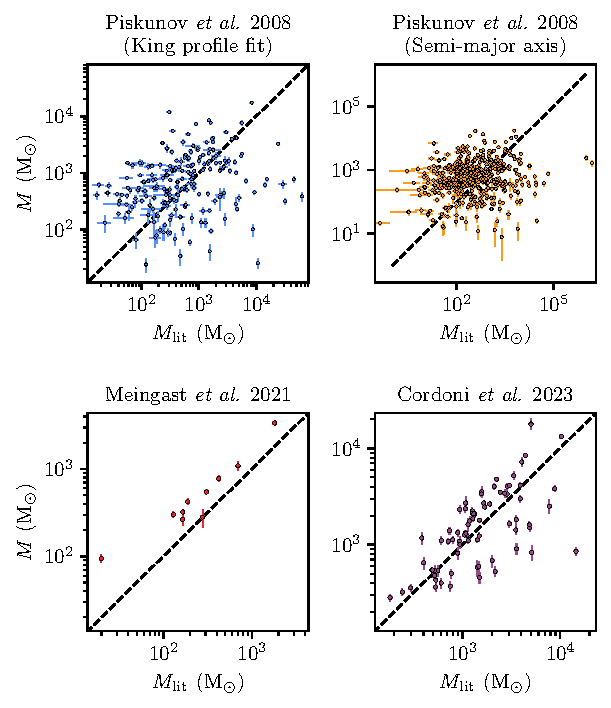
\includegraphics[width=\textwidth]{fig/c4/results_mass_comparison.pdf}
    \caption[Cluster masses derived in this work compared against masses derived in literature works.]{Cluster masses derived in this work compared against masses derived in \cite{piskunov_tidal_2008}, \cite{meingast_extended_2021}, and \cite{cordoni_photometric_binaries_2023} for clusters that appear in both this work and the literature work. Values on the dashed line $y=x$ are in agreement between this work and the literature work.}
    \label{fig:dynamics:results:mass_comparison}
\end{figure}

Masses and Jacobi radii were successfully derived for 6974 clusters in the sample from Paper~2 that are not known globular clusters and are closer than 15~kpc. 72 clusters more distant than this limit have unreliable age and extinction estimates due to their distance not being supported by the age inference neural network from Paper~2. An alternative isochrone fitting method could be used for these objects to derive more accurate age and extinction estimates, before then finding their masses. This would be particularly interesting as it would make it possible to confirm or dispute any potential distant OC discoveries in Paper~2.

There are few cluster mass catalogues in the literature. However, comparison with literature results is still possible on a limited scale. Figure~\ref{fig:dynamics:results:mass_comparison} compares cluster masses derived in this work with masses derived by profile fitting and observations in \cite{piskunov_tidal_2008}, from a similar method to this work in \cite{meingast_extended_2021}, and from \gaia\ DR3 data in \cite{cordoni_photometric_binaries_2023}. 

My results are in some agreement with the work of \cite{meingast_extended_2021}, who apply a similar methodology to ten nearby clusters. However, my masses are generally higher than theirs, which likely arises due to their mass measurements not being corrected for incompleteness. The cluster with the largest disagreement is Platais~9, for which \cite{meingast_extended_2021} find has almost no stars within its Jacobi radius and derive a low bound mass of just 13.1~\MSun, which is significantly lower than my mass measurement of $94.2 \pm 10.3$~\MSun.

Agreement with other works is generally worse. My masses are much larger than the profile-based masses derived in \cite{piskunov_tidal_2008}, although a similar upwards trend exists for some clusters. To derive their masses, the authors used two methods. Firstly, they fit King profiles to 236 clusters in the All Sky Compiled Catalogue 2.5 \cite{kharchenko_allsky_compiled_2001}. Then, assuming that the \cite{king_structure_star_1962} tidal radius $r_t$ is equivalent to $r_J$, one can derive a cluster mass from a profile fit given Eqn.~\ref{eqn:intro:jacobi_radius}. However, this method is extremely sensitive to the adopted cluster radius, since $M_J \propto r_J^3$. As noted in Sect.~\ref{sec:dynamics:masses:jacobi}, there are some cases (such as Ruprecht~134) where my derived Jacobi radius is larger than the observed extent of the cluster -- this is the case for 1195 clusters in the catalogue. Given the depth and quality of \gaia\ data, with cluster membership lists in Paper~2 containing on average around four times as many stars as those in \cite{kharchenko_global_2013}, a plausible explanation for this mass value mismatch would be that many clusters in \cite{piskunov_tidal_2008} may have smaller radii than in this work. On average, King tidal radii derived in Paper~2 are $\approx 1.5\times$ larger than those in \cite{piskunov_tidal_2008}, corresponding to mass estimates that would be $\sim 3\times$ larger in this work. In addition, \cite{piskunov_tidal_2008} also fit semi-major axes to a larger sample of 650 clusters and used these as a proxy for cluster tidal radii, for which my masses have even less correlation.

\cite{cordoni_photometric_binaries_2023} recently created a catalogue of OC masses for 78 clusters by fitting bespoke mass functions to the observed counts of stars for clusters in their sample. For some clusters, my masses are in mild agreement with their results, although my masses are generally higher as \cite{cordoni_photometric_binaries_2023} do not incorporate a correction for CMD incompleteness. However, there are other clusters for which their masses are extremely different to those derived in this work. Haffner~26 is the cluster with the highest reported mass in their work, with a total mass from their mass function fit of 14563~\MSun, which is extremely discrepant with the $852\pm83$~\MSun value of the mass derived for Haffner~26 in this work. In \cite{cordoni_photometric_binaries_2023}, they fit bespoke mass functions to every cluster. For Haffner~26, they fit a steep power law with an overall value of 3.37 above 1~\MSun and 4.78 below 1~\MSun, which is significantly steeper than a Kroupa IMF. Given the reasonably high distance to the cluster of $\sim 3$~kpc, not much of the cluster's low mass regime is resolved in \gaia\ data, and extrapolation of such a steep mass function to unobserved low mass stars is likely to be the reason why their value is so much higher than in this work. While potentially less accurate in some cases for nearby clusters, assumption of a Kroupa IMF for all clusters is at least consistent, and avoids errors in extrapolating steep mass functions to stars that are not observed within a cluster. Nevertheless, the mass function for Haffner~26 within its Jacobi radius in this work appears consistent with a Kroupa IMF down to 0.7~\MSun, suggesting that the steep power law coefficients in \cite{cordoni_photometric_binaries_2023} for this cluster may also be incorrect.

\begin{figure}[t]
    \centering
    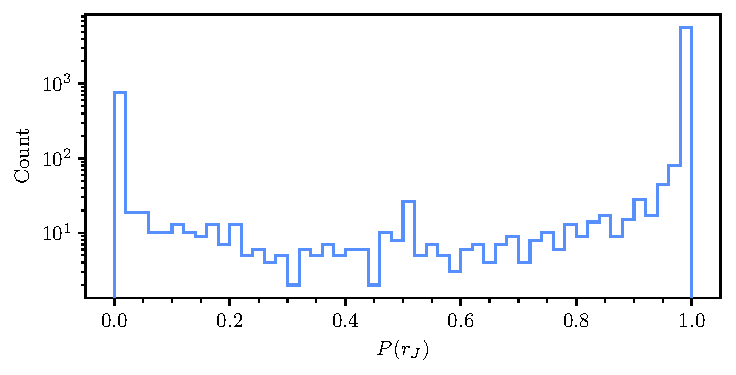
\includegraphics[width=\textwidth]{fig/c4/results_p_jac_distribution.pdf}
    \caption[The distribution of probabilities that a cluster has a valid Jacobi radius]{The distribution of probabilities that a cluster has a valid Jacobi radius for all clusters within 15~kpc.}
    \label{fig:dynamics:results:jacobi_radii_distribution}
\end{figure}

\begin{figure}[t]
    \centering
    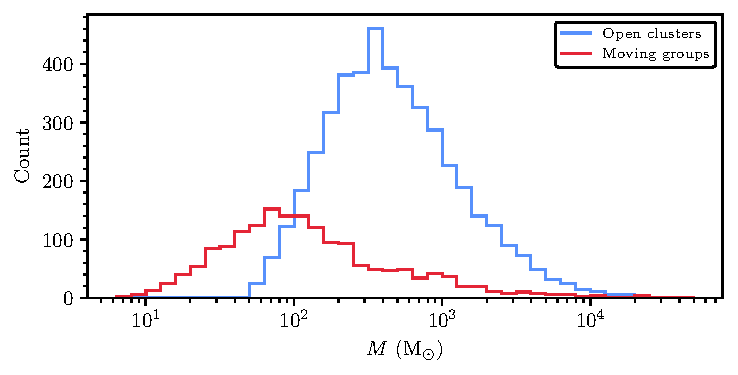
\includegraphics[width=\textwidth]{fig/c4/results_mass_distribution.pdf}
    \caption[The distribution of total masses for all clusters with mass measurements]{The distribution of total masses for all clusters with mass measurements and excluding globular clusters. Clusters are split into samples based on the probability that they have a valid Jacobi radius. In addition, solid lines show this for the `high quality' sample of clusters from Paper~2 (those with an astrometric S/N greater than $5\sigma$ and a median CMD class greater than 0.5), while dashed lines include all clusters with mass measurements in this work.}
    \label{fig:dynamics:results:mass_distribution}
\end{figure}

Having compared masses derived in this work to those derived in the literature, it is next interesting to comment on the overall distribution of results for clusters in this work. Figure~\ref{fig:dynamics:results:jacobi_radii_distribution} shows the distribution of probabilities that a cluster has a valid Jacobi radius, $P(r_J)$. Around 1000 clusters are strongly incompatible with having a bound component, with $P(r_J)\approx0$. On the other hand, around 6000 clusters are strongly compatible with having a valid Jacobi radius, with a handful of clusters taking middling values where they may or may not have a valid $r_J$.

Some moving groups in the Solar neighbourhood appear to have been identified as having a possible valid Jacobi radius, for instance in the densest part of the beta Tucanae moving group detected in Paper~2. The Jacobi masses of these moving groups are generally less than 50~\MSun, with some being lower than 20~\MSun. It is likely that these Jacobi radii are errors. In assuming that all clusters have a mass distribution well-described by a Kroupa IMF, the cluster masses in this work are a more lenient upper limit on the mass of evolved, older systems that may have already lost a number of low-mass stars. Given this method, dynamically evolved moving groups that have lost much of their low-mass content will have an overestimated mass, particularly in their densest regions -- leading to a Jacobi radius being erroneously identified. In addition, the Jacobi radius equation (Eqn.~\ref{eqn:intro:jacobi_radius}) can only be accurately applied on spherically symmetric clusters. Many of these small components of moving groups are not spherically symmetric or have low member counts, which may violate basic assumptions of this method \citep{binney_galactic_1987}. Hence, in deciding which objects are or are not bound OCs, I suggest that an additional minimum $M_J$ of 50~\MSun is adopted, since this is already a mass lower than those of almost any known and reliable OC and removes edge cases where the method simply may not work. Moving groups with a possible Jacobi radius should still be flagged separately in the final catalogue, however, and would also be interesting follow-up candidates for further study of their structure, as a moving group with a core that does have a small Jacobi radius could be a remnant of a dissolved OC.

Figure~\ref{fig:dynamics:results:mass_distribution} shows the distribution of total cluster masses for all clusters in the sample, including comparing these masses against clusters in both the high and low quality samples of clusters in Paper~2. The overall mass distribution of clusters is well characterised by two components, with OC masses centred on a modal mass of around $\sim500$~\MSun and moving group masses centred on a mass of $\sim75$~\MSun. 

In total, masses and Jacobi radii derived in this work appear to be consistent with literature works where relevant, and also show promise in discriminating between clusters that plausibly and implausibly have a gravitational potential stronger than that of the Milky Way, hence implying that they are compatible with bound objects. Next, I review the measurements of virial ratios, which incorporate velocity dispersions to derive a second test for how bound cluster candidates are. 


\subsection{Virial ratios and binary star contamination}
\label{sec:dynamics:results:virial}

I calculated velocity dispersions for all clusters within 15~kpc using the method outlined in Sect.~\ref{sec:dynamics:velocities} and for all stars within the identified Jacobi radius of each cluster, in addition to all stars within an entire cluster. Then, computing the median radius from the cluster centre for stars within the Jacobi radius, I computed corresponding virial ratios of each cluster for both the entire cluster and purely the stars within $r_J$, deriving virial ratios $Q_A$ and $Q_J$ for the entire cluster and for only member stars within $r_J$ respectively.

The distribution of cluster virial ratios as a function of $M_J$ is shown in the upper plot of Fig.~\ref{fig:dynamics:results:virial_vs_mass} for reliable clusters with valid Jacobi radii within 2~kpc. A clear trend is apparent, with $Q_J$ increasing for clusters of lower $M_J$ in an approximately log-linear relation. These results suggest that almost all clusters in the sample appear to be supervirial, with almost no clusters having an observed virial ratio lower than 1 (i.e. twice the ideal value).

\begin{figure}[t]
    \centering
    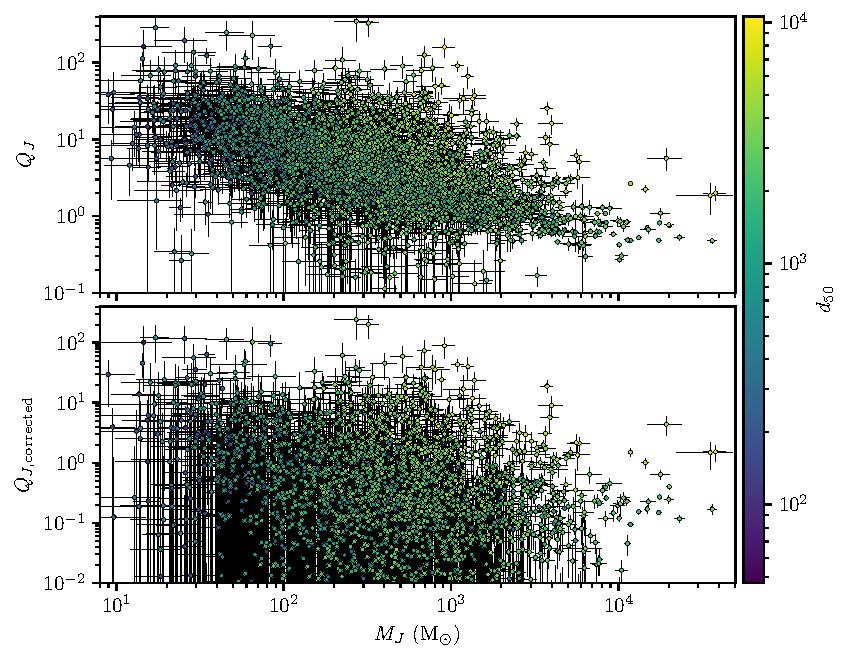
\includegraphics[width=\textwidth]{fig/c4/results_virial_vs_mass.pdf}
    \caption[Virial ratios as a function of mass for all clusters with $P(r_J) > 0.5$]{Virial ratios as a function of mass for all 2030 clusters with $P(r_J) > 0.5$ that are in the high-quality sample of clusters from Paper~2 and that are within~2kpc. Points are shaded based on the median distance to the cluster $d_{50}$. In the upper plot, virial ratios measured for all stars within the cluster's Jacobi radius are shown. In the bottom plot, an approximate correction for dispersion increase arising from unresolved binary stars was applied. On both plots, the dashed red line shows the ideal value of the virial ratio for cluster in dynamical equilibrium, $Q=0.5$.}
    \label{fig:dynamics:results:virial_vs_mass}
\end{figure}

To a certain extent, this mirrors results of recent studies into OC dynamics. For instance, \cite{bravi_gaia-eso_2018}, \cite{kuhn_kinematics_2019}, and \cite{pang_3d_2021} have all found that almost all OCs they studied appear to be supervirial, which is compatible with OCs all being dynamically heated and tidally disrupted by the Milky Way's potential, as is expected for OCs in the disk \citep{krause_physics_2020}. However, the presence of such a clear trend in $Q_J$ as a function of mass is somewhat remarkable, and warrants further investigation.

To begin with, it is worth noting clear flaws in the assumption of a single component Gaussian model for cluster velocity dispersions. Most clusters have tidal tails, implying that stars are being ejected from within the main bound part of the cluster due to tidal interactions with the Milky Way \citep{meingast_extended_2021,tarricq_structural_2022}. In the most extreme cases, a number of nearby clusters such as Melotte~25 (the Hyades) and Platais~9 show heavy ongoing disruption, with their tidal tails containing significantly more mass than the clusters themselves \citep{oh_kinematic_modelling_2020,meingast_extended_2021}. Even within the Jacobi radius, many stars should be being ejected from within the cluster, which will cause an inflation of the mean cluster velocity dispersion. 

A two-component model for cluster velocity dispersions may be more appropriate for such disrupting clusters \citep[see e.g.][]{kuhn_kinematics_2019}, with a component for both bound and unbound stars. However, it may be extremely difficult to reliably differentiate between bound stars and stars undergoing ejection, and such a method is certainly unlikely to be applicable to small or distant clusters with only a few dozen member stars, for which it would be difficult to tell whether a two-component model is a better fit or simply a case of overfitting.

Another explanation for the observed high virial ratios may be unresolved binary stars. Unresolved binaries have been shown to contribute to inflation of cluster radial velocity dispersions in multiple works \citep[e.g.][]{gieles_velocity_2010,rastello_effect_binarity_2020}, with dynamical mass estimates in the worst cases potentially being inflated by factors of 10 to 45 (of which dynamical masses have the same $\sigma_\text{1D}^2$ dependence as $Q$). However, the effect of unresolved binaries on proper motion-derived cluster velocity dispersions has been minimally studied, with a number of important differences and difficulties being present.


\subsubsection{Unresolved binaries as an explanation for high cluster virial ratios}

Unresolved binary star systems can have proper motions perturbed from their true value depending on a number of factors \citep{penoyre_binary_2020}. The principal difference between radial velocity binary contributions and proper motion binary contributions is their mechanism. For a radial velocity to be perturbed, spectral line shifts or broadening due to the orbital motion of binaries contributes directly to the measured radial velocity excess \citep{gieles_velocity_2010}. For instance, a star in a binary pair with a 1~\kms\ orbital speed along the line of sight will have a radial velocity overestimated by $\sim1$~\kms\ relative to the barycentre of the system.

\begin{figure}[t]
    \centering
    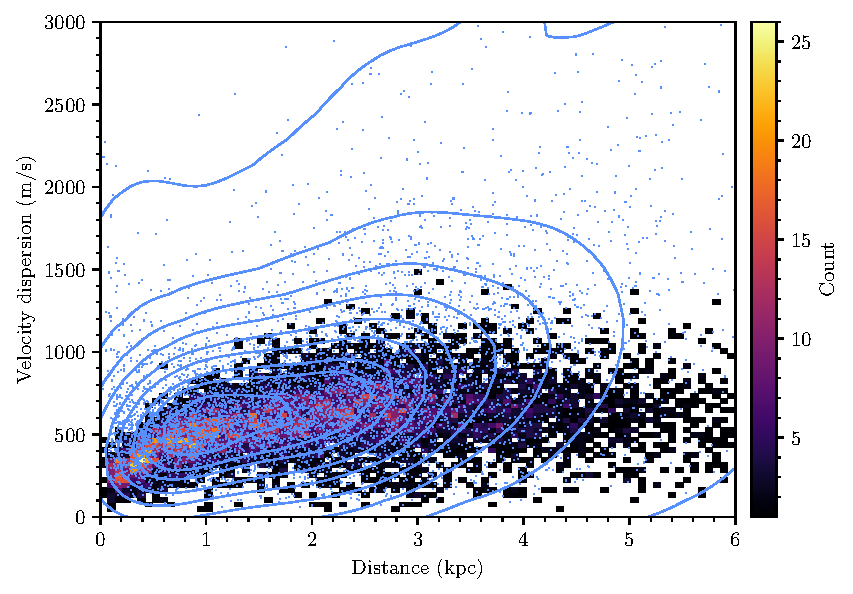
\includegraphics[width=\textwidth]{fig/c4/dispersion_binaries.pdf}
    \caption[Simulated binary star velocity dispersion contaminations as a function of distance for all clusters in the sample]{Simulated binary star velocity dispersion contaminations as a function of distance for all clusters in the sample. Cluster binary star contaminations are shown as a two-dimensional histogram, with bin shading giving the number of clusters in each bin. The measured velocity dispersion of all clusters is shown as a blue contour plot above this histogram.}
    \label{fig:dynamics:velocities:binary_contamination}
\end{figure}

\begin{figure}[t]
    \centering
    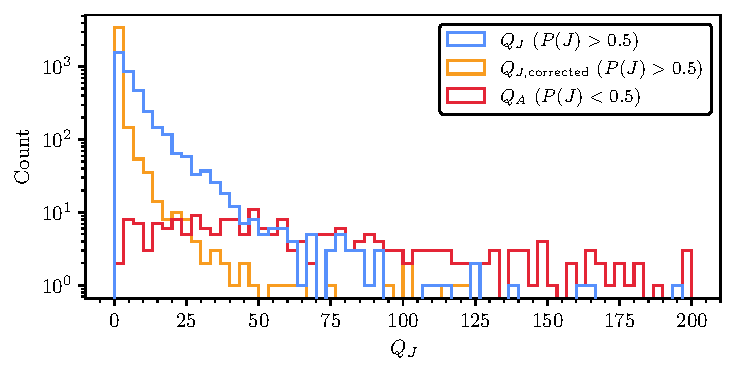
\includegraphics[width=\textwidth]{fig/c4/results_q_distribution.pdf}
    \caption[Distribution of cluster virial ratios]{Distribution of cluster virial ratios. The blue histogram shows virial ratios for clusters with a valid Jacobi radius, the orange histogram shows virial ratios for the same clusters with an approximate correction for binarity applied, and the red histogram shows the virial ratio of the entire cluster for clusters without a valid Jacobi radius.}
    \label{fig:dynamics:results:virial_ratio_distribution}
\end{figure}

However, in the case of an unresolved binary with a proper motion excess, it is the centre of light of the binary system that moves, and not an individual star. This incurs a number of important differences \citep{penoyre_binary_2020}. For instance, an equal mass binary star will have little to no proper motion perturbation, as the centre of light of the system observed by \gaia\ will not move throughout the binary star's orbit. On the other hand, for unequal mass binaries with mass ratios not equal to unity, each star will orbit the barycentre of the binary system at a different radius, causing the centre of light of the system to shift throughout the orbit of the binary and be measured as a shift in the unresolved binary's position over time. This also means that only a small subset of binaries that will impact a cluster's velocity dispersion can be detected with photometric methods, such as those in \cite{cordoni_photometric_binaries_2023} or \cite{donada_multiplicity_fraction_2023}, as these methods are generally only viable in detecting binaries with mass ratios greater than $\sim0.6$, although many binary stars with lesser mass ratios will exist within OCs and will contribute a larger overall amount to OC velocity dispersion inflation.

Proper motion excesses or anomalies have been used by a number of works intentionally to derive catalogues of astrometric binary stars, generally focusing on those within the immediate solar neighbourhood \citep{kervella_stellar_substellar_2019,penoyre_astrometric_2022-1}. However, astrometric binaries within clusters have not yet been studied with \gaia\ data to the best of my knowledge.

To approximately estimate the possible extent of binary star contamination in my derived velocity dispersions, I used \texttt{astromet} \citep{penoyre_astrometric_2022,penoyre_astrometric_2022-1} and \texttt{SPISEA} \citep{hosek_jr_pypopstar_2020} to simulate the clusters studied in this work and their velocity dispersion excess given mean binary star parameters (such as period and eccentricity) for field stars given in \cite{moe_mind_2017}. Both single and binary star astrometry was simulated with \texttt{astromet}. Then, velocity dispersions were measured for these simulated clusters using the pipeline described in Sect.~\ref{sec:dynamics:velocities}.

Figure~\ref{fig:dynamics:velocities:binary_contamination} shows the binary contamination for each cluster as a function of distance. Binary star contamination is lowest for nearby clusters, which have CMDs with deep photometry dominated by lower mass stars, which are expected to have significantly lower chances of being in binary systems than higher mass stars \citep{moe_mind_2017}. This causes the overall velocity dispersion excess at nearby distances to be lower. On the other hand, clusters at distances greater than around 2~kpc have the highest estimated binary star dispersion excess, as their CMDs are dominated by higher mass stars which are expected to mostly be multiple star systems. 

The measured velocity dispersions of clusters in the sample are also overplotted as contours in Fig.~\ref{fig:dynamics:velocities:binary_contamination}, and surprisingly, many clusters have velocity dispersions that are compatible with being almost entirely due to binary star contamination. These simulations are very approximate, and do not include effects such as the evolution of binary star orbital parameters as a function of age.

For the sample of clusters in this work, these simulations are likely to be an overestimate, since cluster selection functions derived in Sect.~\ref{sec:dynamics:masses:selection} suggest that many clusters are missing stars at all magnitudes, which are likely to be binaries with poor quality astrometry that was rejected by the \cite{rybizki_classifier_2022} cut, in addition to the cut on stars with RUWE values greater than 1.4 in velocity dispersion inference (Sect.~\ref{sec:dynamics:velocities:inference}). Nevertheless, they challenge the validity of results showing that most (or even all) clusters are supervirial, and suggest that more work should be done to estimate the excess velocity dispersion that binary stars may contribute to OC proper motion dispersions. 

Motivated by these simulations, I tried a number of methods to remove binary stars from velocity dispersion inference. \cite{penoyre_astrometric_2022,penoyre_astrometric_2022-1} show that cuts on unit weight error, RUWE, or a renormalised local version of the RUWE can be effective in identifying astrometric binaries. However, lowering of the RUWE cut to 1.25 or even 1.0 used in velocity dispersion inference only lowered cluster velocity dispersions by around $\sim10$\%. These approximate methods based on \gaia\ diagnostic criteria are likely imperfect, and may miss many binary stars with periods longer than a few years that can still contribute significantly to cluster velocity dispersions, or with mass ratios that make it too difficult to detect them from astrometry alone.

As an example, Melotte~22 (the Pleiades) is a relatively archetypal cluster, with a mass of $\approx10^3$~\MSun\ and $r_{50}\approx 2.5$~pc. According to Eqn.~\ref{eqn:intro:virial_ratio}, such a cluster should have an ideal velocity dispersion of just 415~\ms. It is easy to simulate scenarios in which a remainder of undetected unresolved binary stars could still contribute even just 100~\ms\ of extra dispersion to a cluster's velocity dispersion, resulting in a virial ratio which is $\sim$50\% larger than the ideal value.

It may not be possible to conclusively remove the impact of unresolved binary stars on cluster velocity dispersions until at least \gaia\ DR4. DR4 is expected to contain significantly more non-single star solutions than \gaia\ DR3 \citep{gaia_collaboration_gaia_2022}.

For comparison, Fig.~\ref{fig:dynamics:results:virial_ratio_distribution} shows the distribution of virial ratios of clusters as measured for those with a valid Jacobi radius, for those without a valid Jacobi radius, and after subtracting estimated binary star contaminations from cluster velocity dispersions by assuming that the true dispersion $\sigma_\text{c,true}=\sqrt{\sigma_\text{c,measured}^2 - \sigma_\text{binary}^2}$, where $\sigma_\text{binary}$ is the simulated binary star contribution for the cluster. In addition, Fig.~\ref{fig:dynamics:results:virial_vs_mass} shows approximately corrected virial ratios as a function of mass, showing that the trend towards higher $Q_J$ values for decreasing cluster mass $M_J$ could be explained by unresolved binaries alone, since the trend apparent in $Q_J$ is removed by the approximate binary correction.

Even after approximately correcting for binaries, some clusters still have significantly higher $Q_J$ values than the ideal value of 0.5. For instance, Melotte~25 (the Hyades) has an uncorrected $Q_J=40.1\pm4.5$, with $Q_{J,\text{corrected}}=25.7\pm3.6$. Inspection of the proper motions of stars within its Jacobi radius shows that many member stars within this radius appear to be being ejected from the cluster, shown by their alignment with the cluster tidal tails. As discussed previously, $Q_J$ is hence not an estimate of the virial ratio of the remaining bound members of a cluster, but rather an estimate of the virial ratio of all stars within my estimated $r_J$ for each cluster, which can include a number of disrupting stars. This may make $Q_J$ also useful as a proxy for how strongly a cluster is currently being disrupted.   


% -------------------------------------
\section{Discussion}
\label{sec:dynamics:discussion}

This chapter is a work in progress ahead of the publication of these results, which will hopefully occur within the coming months. However, even at this early stage, it is still possible to discuss some interesting results that come from this work. I begin by quantifying how many bound and unbound clusters are in the catalogue in Paper~2.


\subsection{An updated observational definition of open clusters}
\label{sec:dynamics:discussion:definition}

\begin{table}[t]

% Define first header
\caption{\label{tab:dynamics:catalogue_results}Total counts of clusters with various different criteria.}

\centering
\begin{tabular}{lp{35mm}cc}
\hline\hline
Type & Criteria & Count & (high quality)\tablefootmark{a} \\
\hline

Open cluster (OC) & $P(r_J)\geq0.5$ and\newline$M_J\geq~50$~\MSun & 5619 & 3515\\
- bound OC & $Q_{J,\text{corrected}} < 5$ & 5051 & 3317 \\
- dissolving OC & $5 \leq Q_{J,\text{corrected}} < 50$ & 501 & 190 \\
- unbound OC? & $50 \leq Q_{J,\text{corrected}}$ & 66 & 8 \\
\hline
Moving group (MG) & $P(r_J)~<~0.5$ or\newline$M_J~<~50$~\MSun & 1355 & 559 \\
- no $r_J$ & $P(r_J) < 0.5$ & 961 & 282 \\
- has $r_J$ & $P(r_J) \geq 0.5$ & 374 & 269 \\
\hline
Globular cluster (GC) & in \cite{vasiliev_gaia_2021} & 121 & 21 \\
\hline
Too distant & $d \geq 15$~kpc & 91 & 17 \\
\hline

\end{tabular}

\tablefoot{
\tablefoottext{a}{Number of clusters passing criteria and that are in the high-quality sample of objects from Paper~2, i.e. those with a median CMD class of greater than 0.5 and an astrometric S/N greater than $5\sigma$.}
}

\end{table} 


\begin{figure}[t]
    \centering
    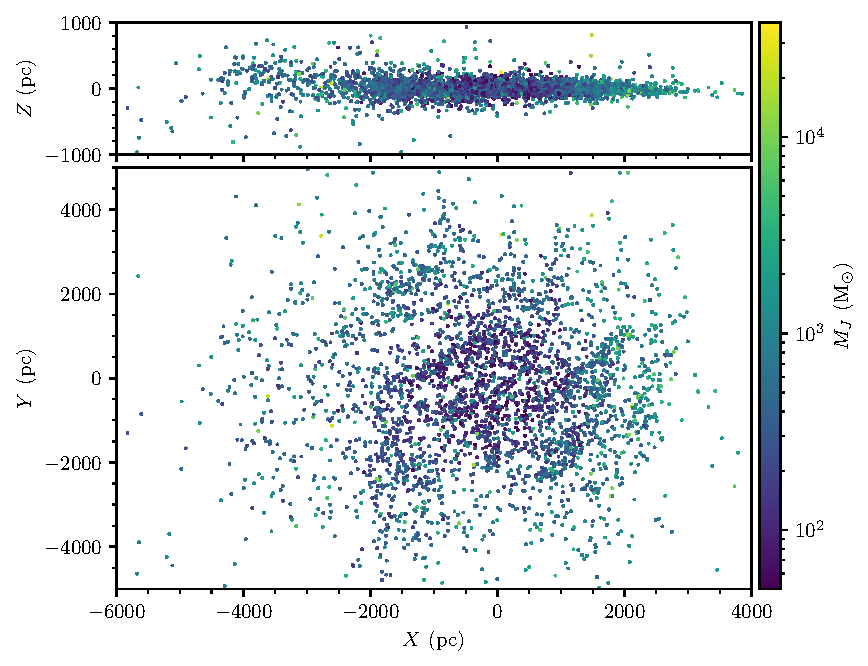
\includegraphics[width=\textwidth]{fig/c4/discussion_xyz_distribution.pdf}
    \caption[Distribution in galactocentric coordinates of 3515 OCs in the high quality sample of OCs]{Distribution in galactocentric coordinates of 3515 OCs in the high quality sample of OCs from Table~\ref{tab:dynamics:catalogue_results}. The Sun is at $X=Y=0$~pc. OCs are shaded by their Jacobi mass.}
    \label{fig:dynamics:discussion:xyz_distribution}
\end{figure}


In Paper~2, we remarked that our catalogue was likely to contain many moving groups. It is now possible to answer how many objects are compatible with moving groups and how many are better characterised as OCs.

The probability of a cluster having a valid Jacobi radius, $P(r_J)$, appears to be a powerful tool in discerning OCs from MGs in our sample from Paper~2. Excluding GCs and 91 clusters more distant than 15~kpc, the total sample of 6974 candidate OCs contains 5619 clusters with $P(r_J)>10$, a minimum mass of 50~\MSun, and at least ten observed stars, representing 82\% of the Paper~2 catalogue. However, most moving groups in Paper~2 appeared to be near to the Sun; within 250~pc, only 32 of 234 clusters (16\%) are compatible with OCs.

Virial ratios derived from cluster velocity dispersions appear much less useful than Jacobi radii for discerning between OCs and MGs, particularly due to the flaws with measured cluster velocity dispersions discussed in Sect.~\ref{sec:dynamics:results:virial}. It is difficult to even choose sensible upper limits on $Q$, as measurements of the virial ratio are likely to be mostly dominated by systematic errors. Systematics due to the $\eta=10$ assumption in Eqn.~\ref{eqn:intro:virial_ratio} can contribute a systematic up to a factor of around two, and simulations of cluster expansion after star formation and during the stellar feedback phase show that star clusters are expected to be supervirial for at least the first 10 to 50~Myr of their lives, and so some degree of superviriality is to be expected for many star clusters \citep{banerjee_how_2017}. 

Assuming that the binary star dispersion corrections from Sect.~\ref{sec:dynamics:results:virial} are even approximately correct, a maximum value of $Q_{J,\text{corrected}}$ of 5 (ten times the ideal value) is probably appropriate, and allows for some amount of superviriality. 5051 clusters pass this limit. A further 501 OCs have $Q_{J,\text{corrected}}$ between 5 and 50, which makes them compatible with OCs that are known to be undergoing strong dissolution -- such as Melotte~25 (the Hyades), for which I measure $Q_{J,\text{corrected}}=25.7 \pm 7.2$. Finally, 66 OCs have $Q_{J,\text{corrected}}\geq50$. These objects may be better classified as MGs due to their extremely high velocity dispersions, which are incompatible with dynamically relaxed objects given even the highest estimated binary star velocity dispersion contamination estimates \citep{rastello_effect_binarity_2020}. Only 8 of these 71 objects also have a median CMD class greater than 0.5 and an astrometric S/N of greater than 5$\sigma$, suggesting that many of the objects with such high virial ratios are simply false positives.

It is also interesting to tally how many of the new objects reported in Paper~2 are compatible with OCs. 1407 of the 2387 newly reported objects in Paper~2 are compatible with OCs. Of the 739 high quality new objects from Paper~2, 469 are also compatible with being OCs.

The overall statistics on total numbers of clusters are shown in Table~\ref{tab:dynamics:catalogue_results}. Counts are shown for both all clusters and clusters that are in the high quality sample from Paper~2.

The distribution of clusters in Paper~2 had a clear maximum in the region a few hundred parsecs around the Sun, due to the many unremoved MGs in the catalogue. Figure~\ref{fig:dynamics:discussion:xyz_distribution} shows the distribution of high-quality OCs in Cartesian coordinates. The distribution around the Sun is relatively uniform out to $\sim1$~kpc, suggesting that the Jacobi radius cut successfully removes most unbound MGs from the catalogue.


\subsection{Completeness of the \gaia\ DR3 open cluster census}
\label{sec:dynamics:results:completeness}

\begin{figure}[t]
    \centering
    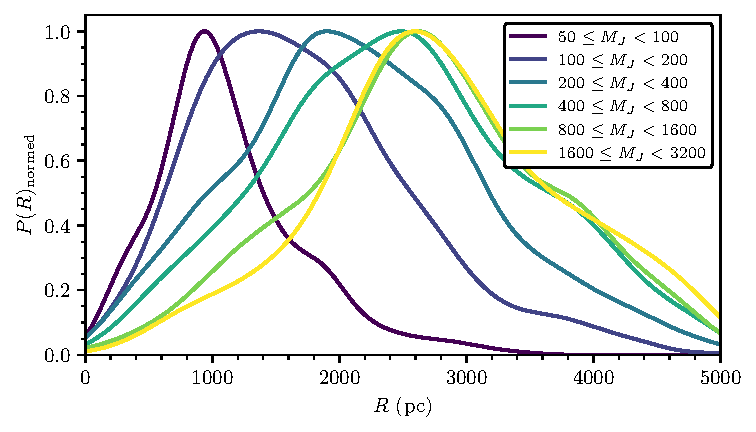
\includegraphics[width=\textwidth]{fig/c4/discussion_completeness.pdf}
    \caption[Distance distribution of the clusters in this work divided into multiple mass bins]{Distance distribution of the clusters in this work divided into multiple mass bins. Cluster distance probability distributions $P(d)$ are smoothed using kernel density estimation, and normalised to all have a peak of one.}
    \label{fig:dynamics:discussion:completeness}
\end{figure}

\begin{figure}[t]
    \centering
    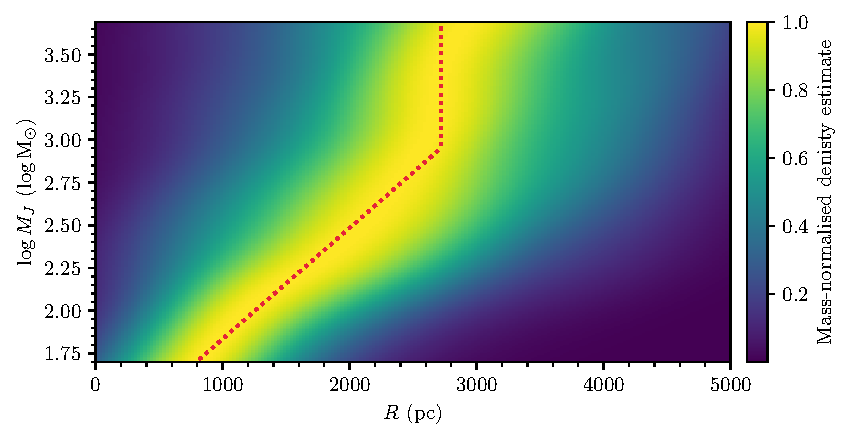
\includegraphics[width=\textwidth]{fig/c4/discussion_completeness_kde.pdf}
    \caption[Mass-distance distribution of clusters shown as a kernel density estimate]{Mass-distance distribution of clusters shown as a kernel density estimate. At a given mass, the density estimate is normalised to have a peak of one, such that every horizontal strip of the diagram is effectively a normalised PDF of cluster distances at a given mass. The dotted red line shows the best fitting log-linear completeness model.}
    \label{fig:dynamics:discussion:completeness_kde}
\end{figure}

\begin{figure}[t]
    \centering
    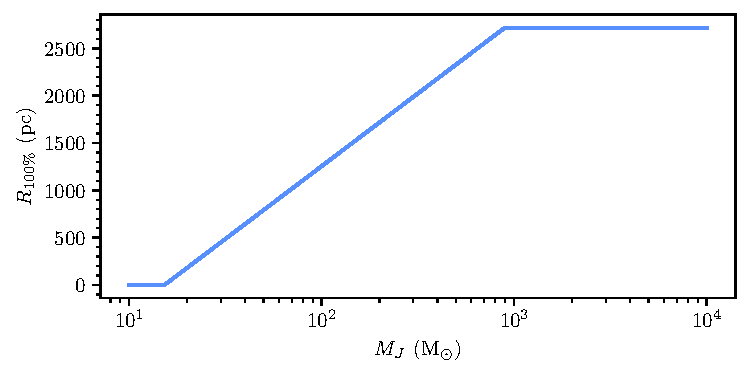
\includegraphics[width=\textwidth]{fig/c4/discussion_completeness_function.pdf}
    \caption[Simple log-linear model for the approximate 100\% completeness limit ($R_{100\%}$) of the cluster census]{Simple log-linear model for the approximate 100\% completeness limit ($R_{100\%}$) of the cluster census as a function of mass.}
    \label{fig:dynamics:discussion:completeness_function}
\end{figure}

Although I have not had much time to analyse the results of this chapter further, one of the most fascinating possible applications of this work would be in deriving the completeness of the \gaia\ DR3 OC census. One of the most widely disproven claims in the \gaia\ era of OC science is that the OC census is not complete within 1.8~kpc \citep{cantat-gaudin_milky_2022}, which is at odds with the catalogue of \cite{kharchenko_global_2013} who derived a completeness limit of 1.8~kpc for the OC census before \gaia. \cite{anders_milky_2020} derived an approximate \gaia\ DR2 OC census completeness limit, but without access to cluster masses, they commented that their completeness estimate was missing a key variable -- it is not known how much the completeness of the OC census depends on mass.

%\todo{below paragraph is poorly explained}
Approximating the distribution of OCs in two dimensions and viewing the Milky Way's disk top-down in Cartesian coordinates, one can define a two-dimensional radius away from the Sun $R=\sqrt{X^2+Y^2}$. The number of OCs in a strip of size $R+\Delta R$ should be proportional to $R$, such that the number of OCs as a function of distance will increase linearly. At some point where incompleteness begins to take effect, this distribution will peak. It should be noted that the distribution of OCs in the galaxy is known to be non-uniform, with imprints of the Milky Way's spiral arms being visible in the distribution of OCs \citep{castro-ginard_milky_2021}: hence, the actual observed distribution of OCs is unlikely to follow this simple model exactly.

Figure~\ref{fig:dynamics:discussion:completeness} shows the $R$ distribution of the OCs identified in this work in multiple mass bins and smoothed using kernel density estimation. The distribution of clusters appears to depend strongly on mass, with clusters at low masses of $50 \leq M_J < 100$~\MSun\ having a peak around 1~kpc, with higher mass clusters with $1600 \leq M_J < 3200$~\MSun\ peaking around 2.6~kpc.

Estimation of the true completeness of the OC census is challenging, as the distribution of OCs depends on some distribution function of OCs in the Milky Way, and cannot be assumed to be uniform \citep{anders_milky_2020}. Deriving such a model for OCs is beyond the scope of this work; however, I can produce a rough estimate of the OC completeness distribution as a function of mass for comparison with other estimates.

Figure~\ref{fig:dynamics:discussion:completeness_kde} shows the mass-$R$ distribution of OCs smoothed with kernel density estimation. To enhance clarity of the peak of this distribution as a function of mass, every horizontal strip is normalised to have a peak of one. Up to a cluster mass of around 1000~\MSun, this distribution appears to be log-linear; for clusters higher than this mass, the peak remains at roughly 2600~pc, suggesting that this is the upper limit of \gaia\ OC completeness for high mass clusters, potentially due to limitations of current DR3 data due to astrometric accuracy or extinction.

I fitted a simple log-linear model to the peak of this distribution, finding the radius at which the DR3 OC census is approximately 100\% complete $R_{100\%}$. This takes the form

\begin{equation}
    R_{100\%} = \alpha \log M_J + \beta
\end{equation}

\noindent
with the additional constraints that $R_{100\%}$ is clipped to be greater than or equal to zero and may not be larger than some value $R_\text{break}$. Fitting to the distribution in Fig.~\ref{fig:dynamics:discussion:completeness_kde}, I find $\alpha=667.8\pm58.2$, $\beta=-1820.3\pm1707.8$, and $R_\text{break}=2720.0\pm69.4$. This approximate fit is shown in Fig.~\ref{fig:dynamics:discussion:completeness_function}. 

In \cite{kharchenko_global_2013}, it was claimed that the OC census is complete within 1.8~kpc. However, based on this simple mass-only model for the completeness of the \gaia\ DR3 OC census, I find that the OC census is only complete within 1.8~kpc for clusters heavier than around 230~\MSun, being incomplete at distances larger than around 1~kpc for clusters at a mass of 100~\MSun.


% -------------------------------------
\section{Conclusion}
\label{sec:dynamics:conclusion}

In this chapter of preliminary results, I aimed to investigate methods to distinguish between bound OCs and unbound MGs. To do so, I derived masses, Jacobi radii, and proper motion dispersions for 6974 clusters from Paper~2, and used these to compute the probabilities that clusters have valid Jacobi radii and have virial ratios compatible with bound objects. I show that it is possible to accurately distinguish between bound OCs and unbound MGs using \gaia\ data.

My mass measurements form the largest catalogue of OC masses to date, being over 70 times larger than the largest catalogue of OC masses made using \gaia\ data. For each cluster, I computed the selection function of its CMD as a function of $G$ magnitude, estimating three separate quantities that contribute towards CMD incompleteness to derive accurate cluster masses. My OC masses are generally higher than results derived in the literature, which is likely due to the addition of these incompleteness estimates.

Using my mass measurement pipeline, I derived Jacobi radii for the sample of clusters. I found that only 82\% of the clusters from Paper~2 are compatible with bound objects that have a valid Jacobi radius, dropping to just 16\% of the clusters in Paper~2 within 250~pc.

In addition, I investigated the virial ratios of the clusters in the catalogue, using the proper motions of member stars to derive cluster proper motion dispersions with a maximum likelihood method. However, I found that \gaia\ proper motions are generally an ineffective tool in distinguishing between bound and unbound objects, as the velocity dispersion of most OCs appears to be compatible with being dominated by dispersion contributions from resolved and unresolved binary stars.

Combining these results, I find that there are 5619 OCs in the catalogue with 3515 being of high quality. Likewise, there are 1355 MGs in the catalogue, 559 of which are of a high quality. I find that cluster Jacobi radii are a particularly effective tool to distinguish between bound OCs and unbound MGs. These results represent a leap forwards in the ability to distinguish between bound and unbound star clusters in the Milky Way: by applying relatively simple physical laws governing the dynamics of star clusters, I am able to show with significantly higher accuracy which objects are and are not bound compared to previous empirical methods.

Finally, I use these results to derive tentative approximate estimates of the completeness of the OC census in \gaia\ DR3. I find that the completeness of the census is well described by a logarithmic function until a distance around 2700~pc, at which the 100\% completeness limit does not increase higher with increasing OC mass. Within 1.8~kpc, the OC census only appears approximately complete for OCs heavier than around 230~\MSun.
